\documentclass[]{beamer}

\usepackage[utf8x]{inputenc}        % diacritice
\usepackage[english]{babel}
\usepackage{color}                  % highlight
\usepackage{alltt}                  % highlight
\usepackage{qcircuit}

% Define the logos to be used at the top of the title page
\newcommand{\logopanel}{%
  \makebox[0.40\paperwidth]{%
  \raisebox{-0.05cm}{
\includegraphics[width=1.35cm,keepaspectratio]{./pics/upb.png}}%
    \hspace{0.85cm}%
    \raisebox{-0.15cm}{
\includegraphics[width=2.95cm,keepaspectratio]{./pics/LogoIQC.png}}%
    \hspace{0.35cm}%
    
\includegraphics[width=2.75cm,keepaspectratio]{./pics/cs.png}%
    \hspace{-0.6cm}%
  }%
}

\usefonttheme{default}
\useinnertheme{rounded}

\setbeamertemplate{bibliography item}{\insertbiblabel}

% highlight; comment this out in case you don't input code source files
\usepackage{hyperref}               % folosiți \url{http://...}
                                    % sau \href{http://...}{Nume Link}
\usepackage{verbatim}
\definecolor{UBCblue}{rgb}{0.05706, 0.23725, 0.46667} % UBC Blue (primary)
\definecolor{customblue}{rgb}{0.3, 0.4, 0.7}          % Custom blue color

\usecolortheme[named=UBCblue]{structure}
\mode<presentation>
{ \usetheme{Berlin} }

% Încărcăm simbolurilor Unicode românești în titlu și primele pagini
\PreloadUnicodePage{200}

% Arătăm numărul frame-ului
\newcommand{\frameofframes}{/}
\newcommand{\setframeofframes}[1]{\renewcommand{\frameofframes}{#1}}

\setframeofframes{of}
\makeatletter
\setbeamertemplate{footline}
  {%
    \begin{beamercolorbox}[colsep=1.5pt]{upper separation line foot}
    \end{beamercolorbox}
    \begin{beamercolorbox}[ht=2.5ex,dp=1.125ex,%
      leftskip=.3cm,rightskip=.3cm plus1fil]{author in head/foot}%
      \leavevmode{\usebeamerfont{author in head/foot}\insertshortauthor}%
      \hfill%
      {\usebeamerfont{institute in head/foot}\usebeamercolor[fg]{institute in head/foot}Computer Science and Engineering Department}%
    \end{beamercolorbox}%
    \begin{beamercolorbox}[ht=2.5ex,dp=1.125ex,%
      leftskip=.3cm,rightskip=.3cm plus1fil]{title in head/foot}%
      {\usebeamerfont{title in head/foot}\insertshorttitle}%
      \hfill%
      {\usebeamerfont{frame number}\usebeamercolor[fg]{frame number}\insertframenumber~\frameofframes~\inserttotalframenumber}
    \end{beamercolorbox}%
    \begin{beamercolorbox}[colsep=1.5pt]{lower separation line foot}
    \end{beamercolorbox}
  }
\makeatother

\setbeamertemplate{navigation symbols}{}%remove navigation symbols

% Title page customization
\setbeamertemplate{title page}
{
    \begin{center}
        \logopanel
    \end{center}
    \vspace{0.05cm}  % Adjust this value to reduce the space between logos and title
    \begin{beamercolorbox}[wd=\textwidth,ht=1.6cm,dp=0.00001cm,rounded=true, shadow=true, sep=8pt, center]{title}
        \usebeamerfont{title}\inserttitle\par%
        \ifx\insertsubtitle\@empty%
        \else%
          \vskip0.25em%
          {\usebeamerfont{subtitle}\usebeamercolor[fg]{subtitle}\insertsubtitle\par}%
        \fi%
    \end{beamercolorbox}%
    \vskip1em\par%
    \begin{beamercolorbox}[sep=8pt,center]{author}
        \usebeamerfont{author}\insertauthor
    \end{beamercolorbox}
    \begin{beamercolorbox}[sep=8pt,center]{institute}
        \usebeamerfont{institute}\insertinstitute
    \end{beamercolorbox}
    \begin{beamercolorbox}[sep=8pt,center]{date}
        \usebeamerfont{date}\insertdate
    \end{beamercolorbox}
    \vfill
}

\title[]{}
\subtitle{QRKT-GAN: Neural ODE-Inspired Generative Adversarial Network with Numerical Runge-Kutta Methods for Quantum Visual Transformer-Based Generator and Discriminator}
\institute{Faculty of Automatic Control and Computers,\\
National University of Science and Technology POLITEHNICA Bucharest}
\author[Cătălin-Alexandru Rîpanu (UPB)]{Cătălin-Alexandru Rîpanu \\ Supervisor: Șl. dr. ing. Dumitru-Clementin Cercel}
\date{July 2, 2024}

\begin{document}

% Slide-urile cu mai multe părți sunt marcate cu textul (cont.)
\setbeamertemplate{frametitle continuation}[from second][(\insertcontinuationcount)]

\begin{frame}
  \titlepage
\end{frame}


% NB: Secțiunile nu sunt marcate vizual, ci doar apar în cuprins
\section{Context}

% Titlul unui frame se specifică fie în acolade, imediat după \begin{frame},
% fie folosind \frametitle
\begin{frame}[t]{Context}
  \bigskip
  In Artificial Intelligence, \textbf{Deep Learning} models:
  \smallskip
  \begin{enumerate}
    \visible<2->{
    \item demonstrated \textbf{remarkable results} across various domains:
          \smallskip
          \visible<3->{
            \begin{itemize}
              \item Object Classification (Computer Vision)
                    \smallskip
              \item Image Segmentation (Computer Vision)
                    \smallskip
              \item Sentiment Analysis (Natural Language Processing)
                    \smallskip
              \item Synthetic Data Generation
            \end{itemize}
          }
          }
          \visible<4->{
    \item greatly improved human lives (Medical Image Recognition~\cite{he2020infusing})
          }
  \end{enumerate}
  \bigskip
  \visible<5->{
    however\dots
  }
  \\
  \bigskip
  \visible<6->{
    for such performance \dots \alert{millions to billions of neurons are required}.
  }

\end{frame}

\begin{frame}[t]{Context (2)}
  \bigskip
  Numerous solutions have been developed to mitigate this problem:
  \visible<2->{
  \begin{enumerate}
    \item Grid Search and Random Search~\cite{liashchynskyi2019grid,randomsearch}
          \smallskip

    \item Group Sparsity Regularizers~\cite{alvarez2018learning}
          \smallskip


    \item Dimensionality Reduction and Kernel-Sharing~\cite{wen2021convolutional,azadbakht2022drastically}
          \smallskip


    \item Network Weights Splitting~\cite{pmlr-v70-kim17b}


    \item Particle Swarm Optimization~\cite{7986470}
          }
  \end{enumerate}
  \smallskip
  \smallskip
  \visible<3->{
    unfortunately\dots
  }
  \\
  \smallskip
  \smallskip
  \smallskip
  \visible<4->{
    these \textbf{classical} methods have \alert{inherent drawbacks} in their logic.
  }
\end{frame}

\section{GANs}

\begin{frame}{Generative Adversarial Networks (GANs)}
  \visible<2->{
  \begin{figure}[th]
    \centering
    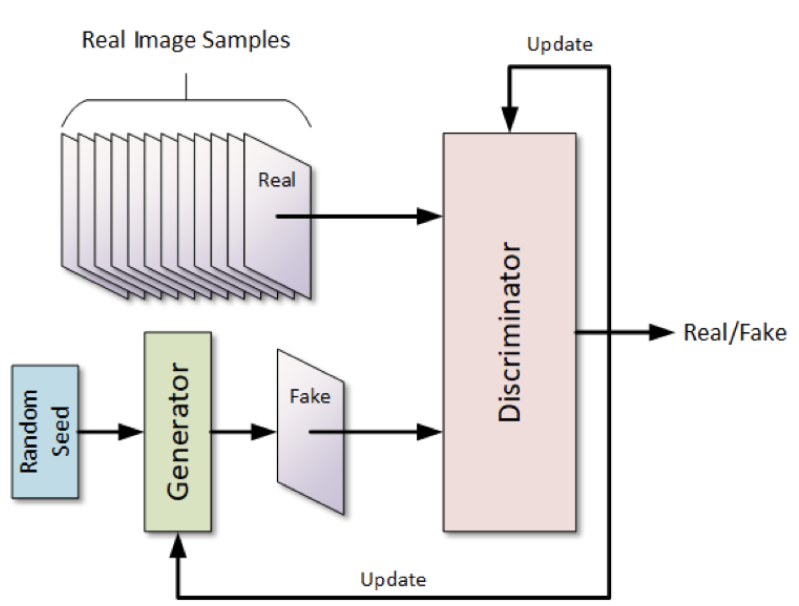
\includegraphics[scale=0.35]{./pics/gan.png}
    \caption[Generative Adversarial Network Architecture]{The Generative Adversarial Network Architecture~\cite{gan-photo}}
    \label{fig:pi1}
    }
  \end{figure}
\end{frame}

\section{Transfomers}

\begin{frame}{The Transformer}
  \visible<2->{
  \begin{figure}[th]
    \centering
    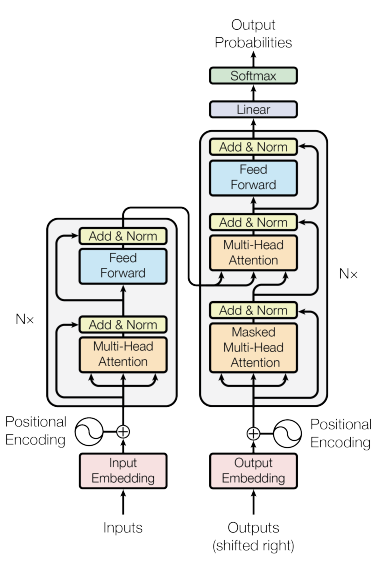
\includegraphics[scale=0.385]{./pics/transformer.png}
    \caption[Transformer Architecture]{The Transformer Architecture~\cite{vaswani2017attention}}
    \label{fig:pi2}
    }
  \end{figure}
\end{frame}

\section{Visual Transfomers}
\begin{frame}{The Visual Transformer}
  \visible<2->{
  \begin{figure}[th]
    \centering
    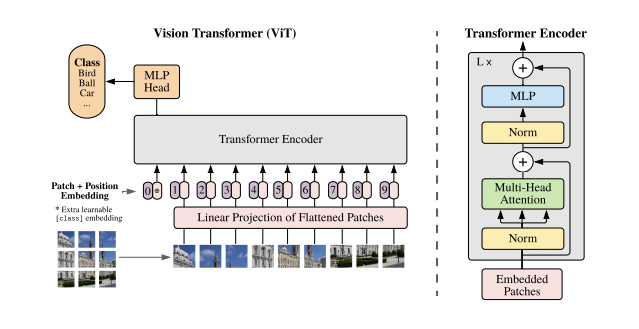
\includegraphics[scale=0.638]{./pics/vit.png}
    \caption[Visual Transformer Architecture]{The Visual Transformer Architecture~\cite{vaswani2017attention, dosovitskiy2020}}
    \label{fig:pi3}
    }
  \end{figure}
\end{frame}

\begin{frame}{The Visual Transformer (2)}
  Thus, the transformation at each layer is defined as:
  \bigskip
  \visible<2->{
    \begin{equation}
      W = X + \text{MHA}(\text{Norm}(X), \text{Norm}(X), \text{Norm}(X))
    \end{equation}

    \begin{equation}
      X' = W + \text{MLP}(\text{Norm}(W))
    \end{equation}

    \bigskip
    where \( X, X' \in \mathbb{R}^{N \times D} \).
  }
\end{frame}

\begin{frame}{The Visual Transformer (3)}
  And\dots the Multi-Head Attention Mechanism can be expressed as:
  \bigskip
  \visible<2->{
    \begin{equation}
      \text{Attention}(V, K, Q) = \text{softmax}\left(\frac{QK^T}{\sqrt{D_k}}\right) V
    \end{equation}

    \begin{equation}
      \text{MHA}(V, K, Q) = \text{Concat}(\text{single\_head}_i) W^O, i=1:h
    \end{equation}

    \begin{equation}
      \text{single\_head}_i = \text{Attention}(V W_i^V, K W_i^K, Q W_i^Q)
    \end{equation}
  }
  \visible<3->{
    \\
    where:
    \begin{itemize}
      \item \( W_i^K \in \mathbb{R}^{D_x \times D_k} \), \( W_i^V \in \mathbb{R}^{D_x \times D_v} \), \( W_i^Q \in \mathbb{R}^{D_x \times D_k} \)
      \item \( W^O \in \mathbb{R}^{h D_v \times D_x} \)
    \end{itemize}
  }
\end{frame}

\begin{frame}{The Visual Transformer (4)}
  Let \( Y^m = [y_1^m, y_2^m, \ldots, y_L^m] \)~\cite{zhong2022neural}:
  \visible<2->{
    \begin{equation}\label{eq:1}
      \hat{y}_i^m = y_i^m + G(y_i^m, Y^m), \quad 1 \leq i \leq L,
    \end{equation}
  }
  \\
  \visible<3->{
  The output \( \hat{Y}^m = [\hat{y}_1^m, \hat{y}_2^m, \ldots, \hat{y}_L^m] \) is then fed to the MLP:

  \begin{equation}\label{eq:2}
    y_i^{m+1} = \hat{y}_i^m + H(\hat{y}_i^m), \quad 1 \leq i \leq L,
  \end{equation}
  }
  \\
  \visible<4->{
    Over the time interval \([m, m+1]\), using Lie-Trotter decomposing method ~\cite{lu2019understanding, dutta2021redesigning}:
    \begin{equation}
      \frac{dy_i}{dt} = H(y_i) + G(y_i, Y)
    \end{equation}
  }
\end{frame}

\section{Runge-Kutta}

\begin{frame}{Neural Runge-Kutta Method (RK4)}
  Let $F(y_i, Y) = H(y_i) + G(y_i, Y)$
  \smallskip
  \\
  \visible<2->{
    In this context, Runge-Kutta method can be written as:
  }
  \visible<3->{
    \begin{equation}
      y_i(t + 1) = y_i(t) + \sum_{j=1}^{n}\gamma_{j}F_{ij}
    \end{equation}
    \begin{equation}
      F(y_i, Y) = F_i
    \end{equation}
    \begin{equation}
      F_{ij} = F_i(y_i + \sum_{p=1}^{j-1}\beta_{jp}F_{ip}, Y)
    \end{equation}
  }
  \visible<4->{
    Thus }
  \visible<5->{
    \begin{equation}
      y_i(t + 1) = y_i(t) + \frac{1}{6}(F_{i1} + 2F_{i2} + 2F_{i3} + F_{i4})
    \end{equation}
  }
\end{frame}

\section{Quantum}

\begin{frame}{The Quantum Visual Transformer}
  \visible<2->{
    \begin{figure}[th]
      \centering
      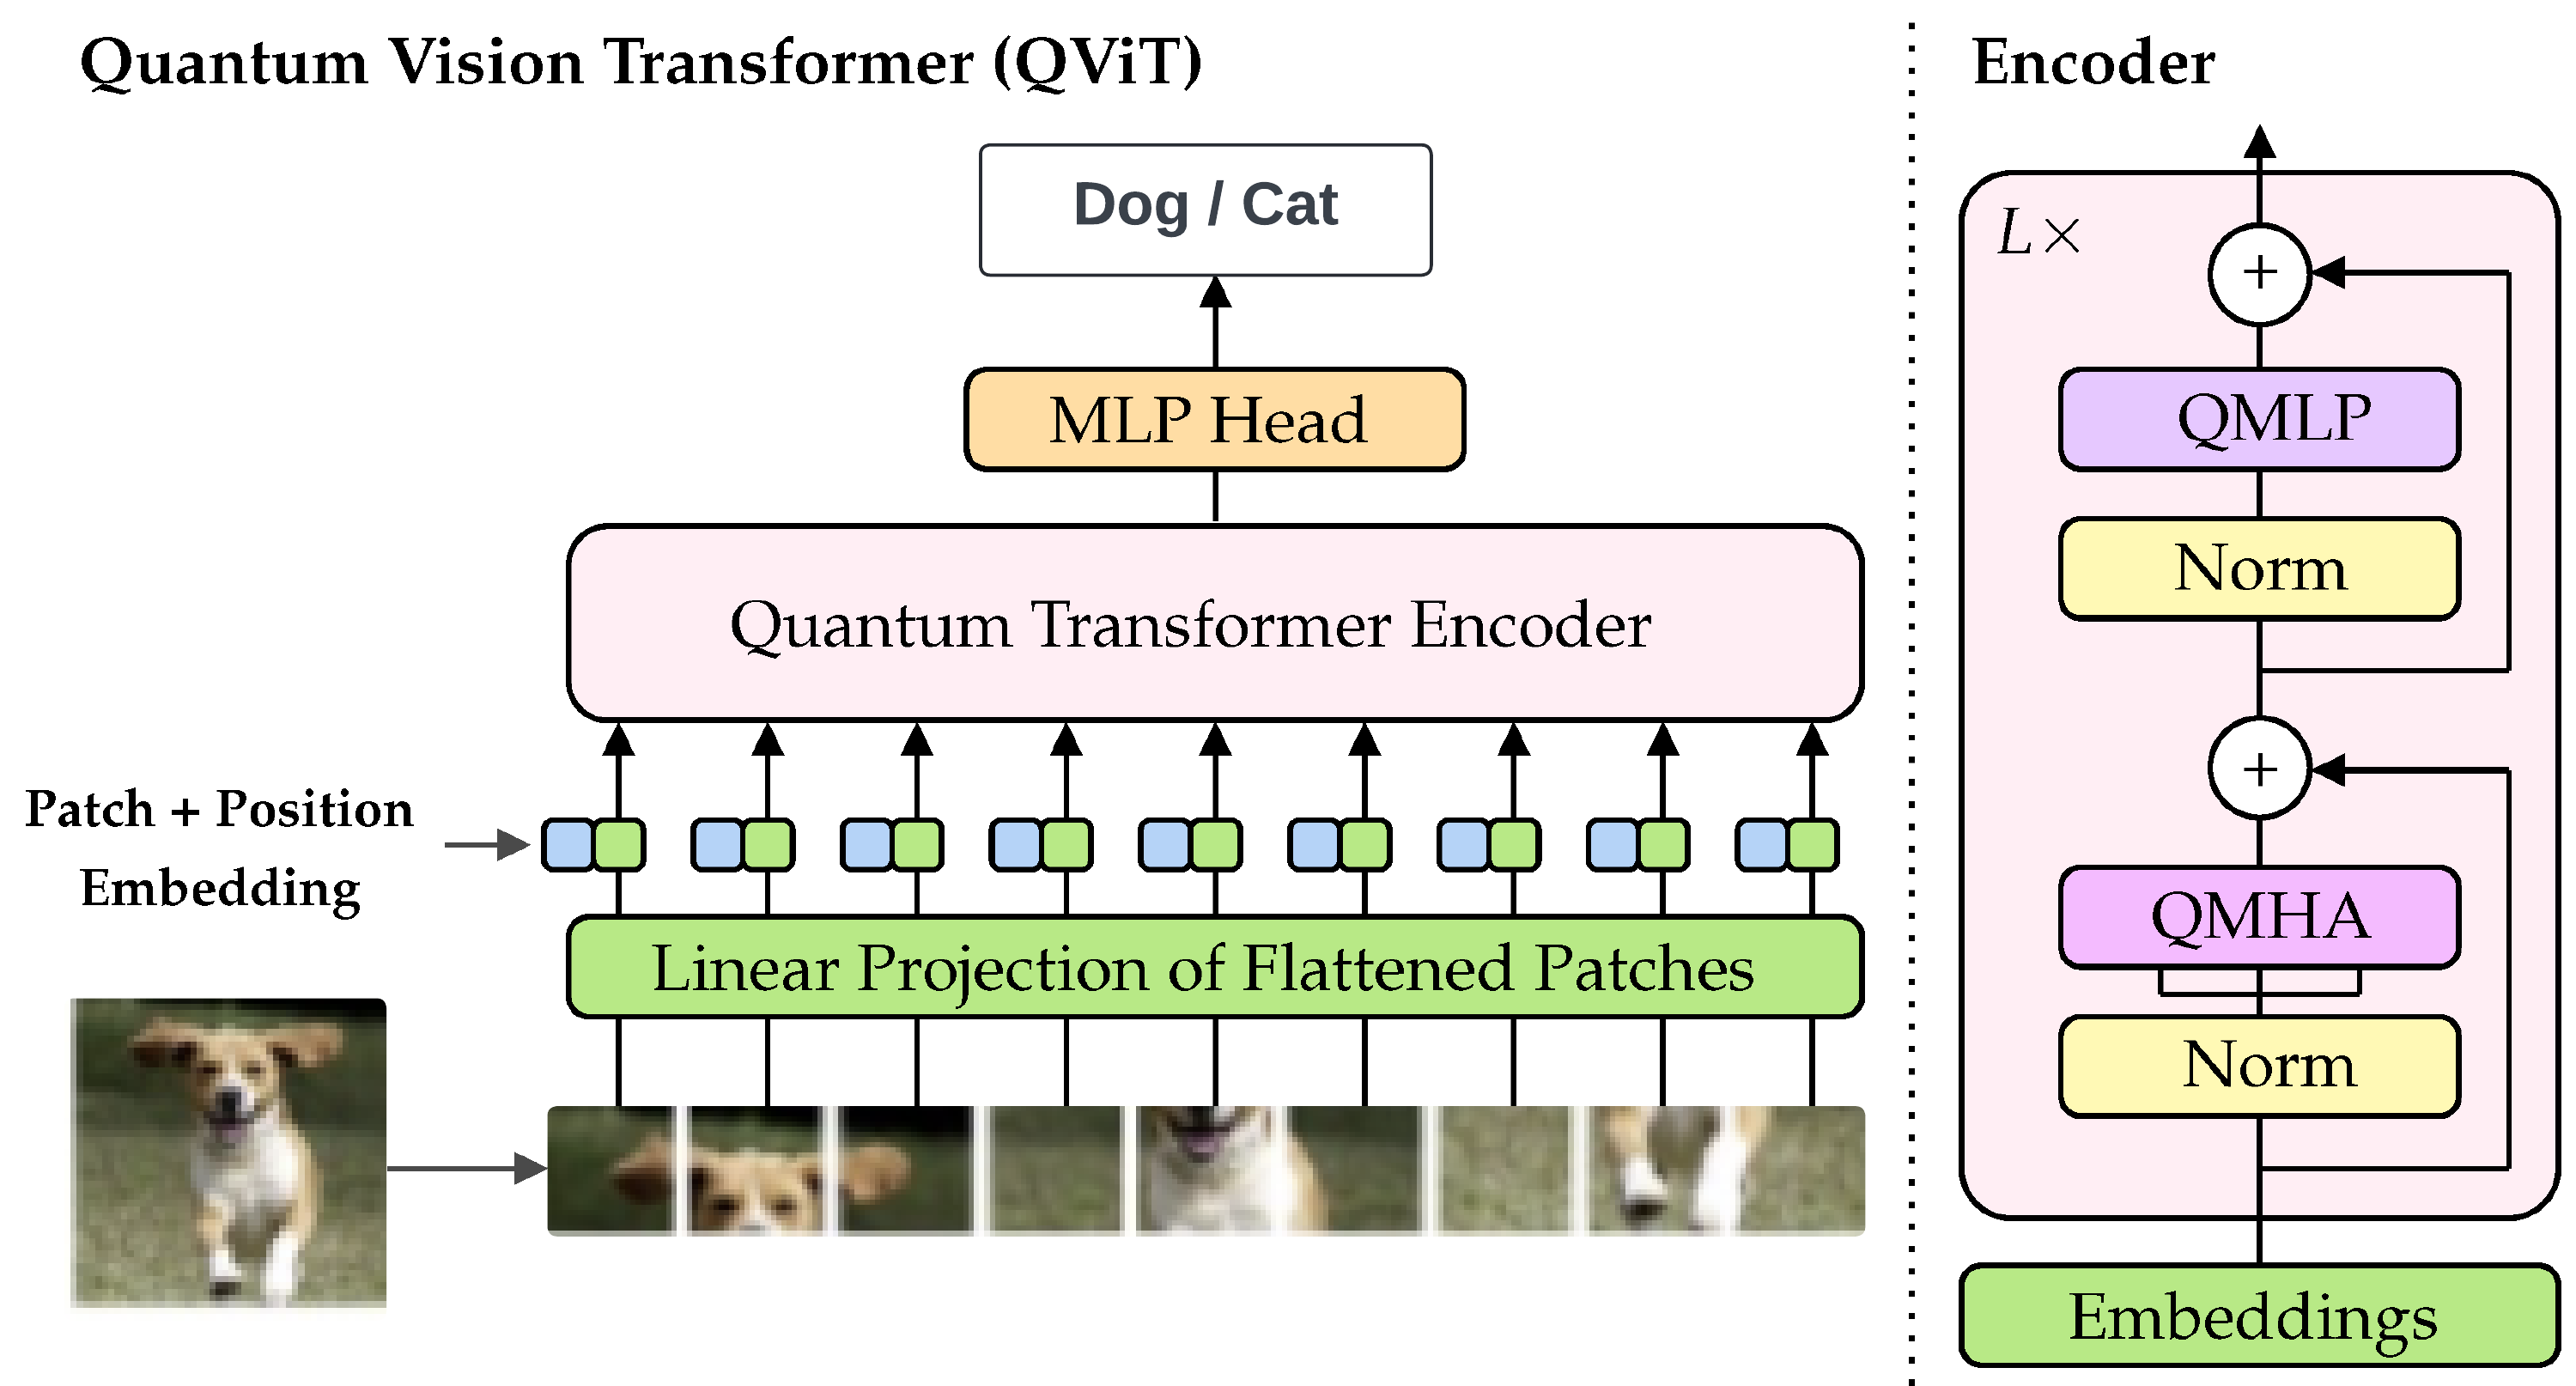
\includegraphics[scale=0.099]{./pics/Blank diagram - Page 1.png}
      \caption[Visual Quantum Transformer]{Visual Quantum Transformer~\cite{Comajoan_Cara_2024}}
      \label{fig:p4}
    \end{figure}
  }
\end{frame}

\begin{frame}{Quantum Gates}
  \visible<2->{
    \begin{minipage}{0.45\textwidth}
      \[
        \text{CNOT} = \begin{bmatrix}
          1 & 0 & 0 & 0 \\
          0 & 1 & 0 & 0 \\
          0 & 0 & 0 & 1 \\
          0 & 0 & 1 & 0
        \end{bmatrix}
      \]
    \end{minipage}
    \hfill
    \begin{minipage}{0.45\textwidth}
      \[
        H = \frac{1}{\sqrt{2}} \begin{bmatrix}
          1 & 1  \\
          1 & -1
        \end{bmatrix}
      \]
    \end{minipage}
    \vspace{1em} % Add some vertical space

    \begin{minipage}{0.45\textwidth}
      \[
        R_X(\theta) = \begin{bmatrix}
          \cos(\theta/2)   & -i\sin(\theta/2) \\
          -i\sin(\theta/2) & \cos(\theta/2)
        \end{bmatrix}
      \]
    \end{minipage}
    \hfill
    \begin{minipage}{0.45\textwidth}
      \[
        R_Z(\theta) = \begin{bmatrix}
          e^{-i\theta/2} & 0             \\
          0              & e^{i\theta/2}
        \end{bmatrix}
      \]
    \end{minipage}
    \vspace{1em} % Add some vertical space
    \begin{minipage}{0.45\textwidth}
      \[
        R_Y(\theta) = \begin{bmatrix}
          \cos(\theta/2) & -\sin(\theta/2) \\
          \sin(\theta/2) & \cos(\theta/2)
        \end{bmatrix}
      \]
    \end{minipage}
  }
\end{frame}

\begin{frame}{The Variational Quantum Circuit}
  One can use such techniques\dots \visible<2->{\alert{only in another reality}.}
  \visible<3->{
    \begin{figure}[h]
      \centering
      \resizebox{1.05\textwidth}{!}{ % Adjust the scaling factor as needed (width set to 80% of text width)
        \ensuremath{ % Ensure math mode is enabled
          \begin{array}{c}
            \Qcircuit @C=0.75em @R=1.1em {
            \lstick{| \psi_0 \rangle}     & \gate{R_y(x_0)}     & \gate{R_x(\theta_0)}     & \gate{R_z(\theta_0)}     & \gate{H} & \ctrl{1} & \qw      & \qw      & \qw      & \qw      & \qw    & \qw      & \qw      & \qw      & \targ     & \meter \\
            \lstick{| \psi_1 \rangle}     & \gate{R_y(x_1)}     & \gate{R_x(\theta_1)}     & \gate{R_z(\theta_1)}     & \qw      & \targ    & \gate{H} & \ctrl{1} & \qw      & \qw      & \qw    & \qw      & \qw      & \qw      & \qw       & \meter \\
            \lstick{| \psi_2 \rangle}     & \gate{R_y(x_2)}     & \gate{R_x(\theta_2)}     & \gate{R_z(\theta_2)}     & \qw      & \qw      & \qw      & \targ    & \gate{H} & \ctrl{1} & \qw    & \qw      & \qw      & \qw      & \qw       & \meter \\
                                          & \vdots              & \vdots                   & \vdots                   &          &          &          &          &          & \vdots   & \vdots &          &          &          &           & \vdots \\
            \lstick{| \psi_{n-2} \rangle} & \gate{R_y(x_{n-2})} & \gate{R_x(\theta_{n-2})} & \gate{R_z(\theta_{n-2})} & \qw      & \qw      & \qw      & \qw      & \qw      & \qw      & \targ  & \gate{H} & \ctrl{1} & \qw      & \qw       & \meter \\
            \lstick{| \psi_{n-1} \rangle} & \gate{R_y(x_{n-1})} & \gate{R_x(\theta_{n-1})} & \gate{R_z(\theta_{n-1})} & \qw      & \qw      & \qw      & \qw      & \qw      & \qw      & \qw    & \qw      & \targ    & \gate{H} & \ctrl{-5} & \meter \\
            }
          \end{array}
        }
      }
      \smallskip
      \caption{The Variational Quantum Circuit used in QRKT-GAN} \label{fig:vqc}
    \end{figure}
  }
\end{frame}

\begin{frame}{Proposed Solution (QRKT-GAN)}
  \visible<2->{
    \begin{figure}[th]
      \centering
      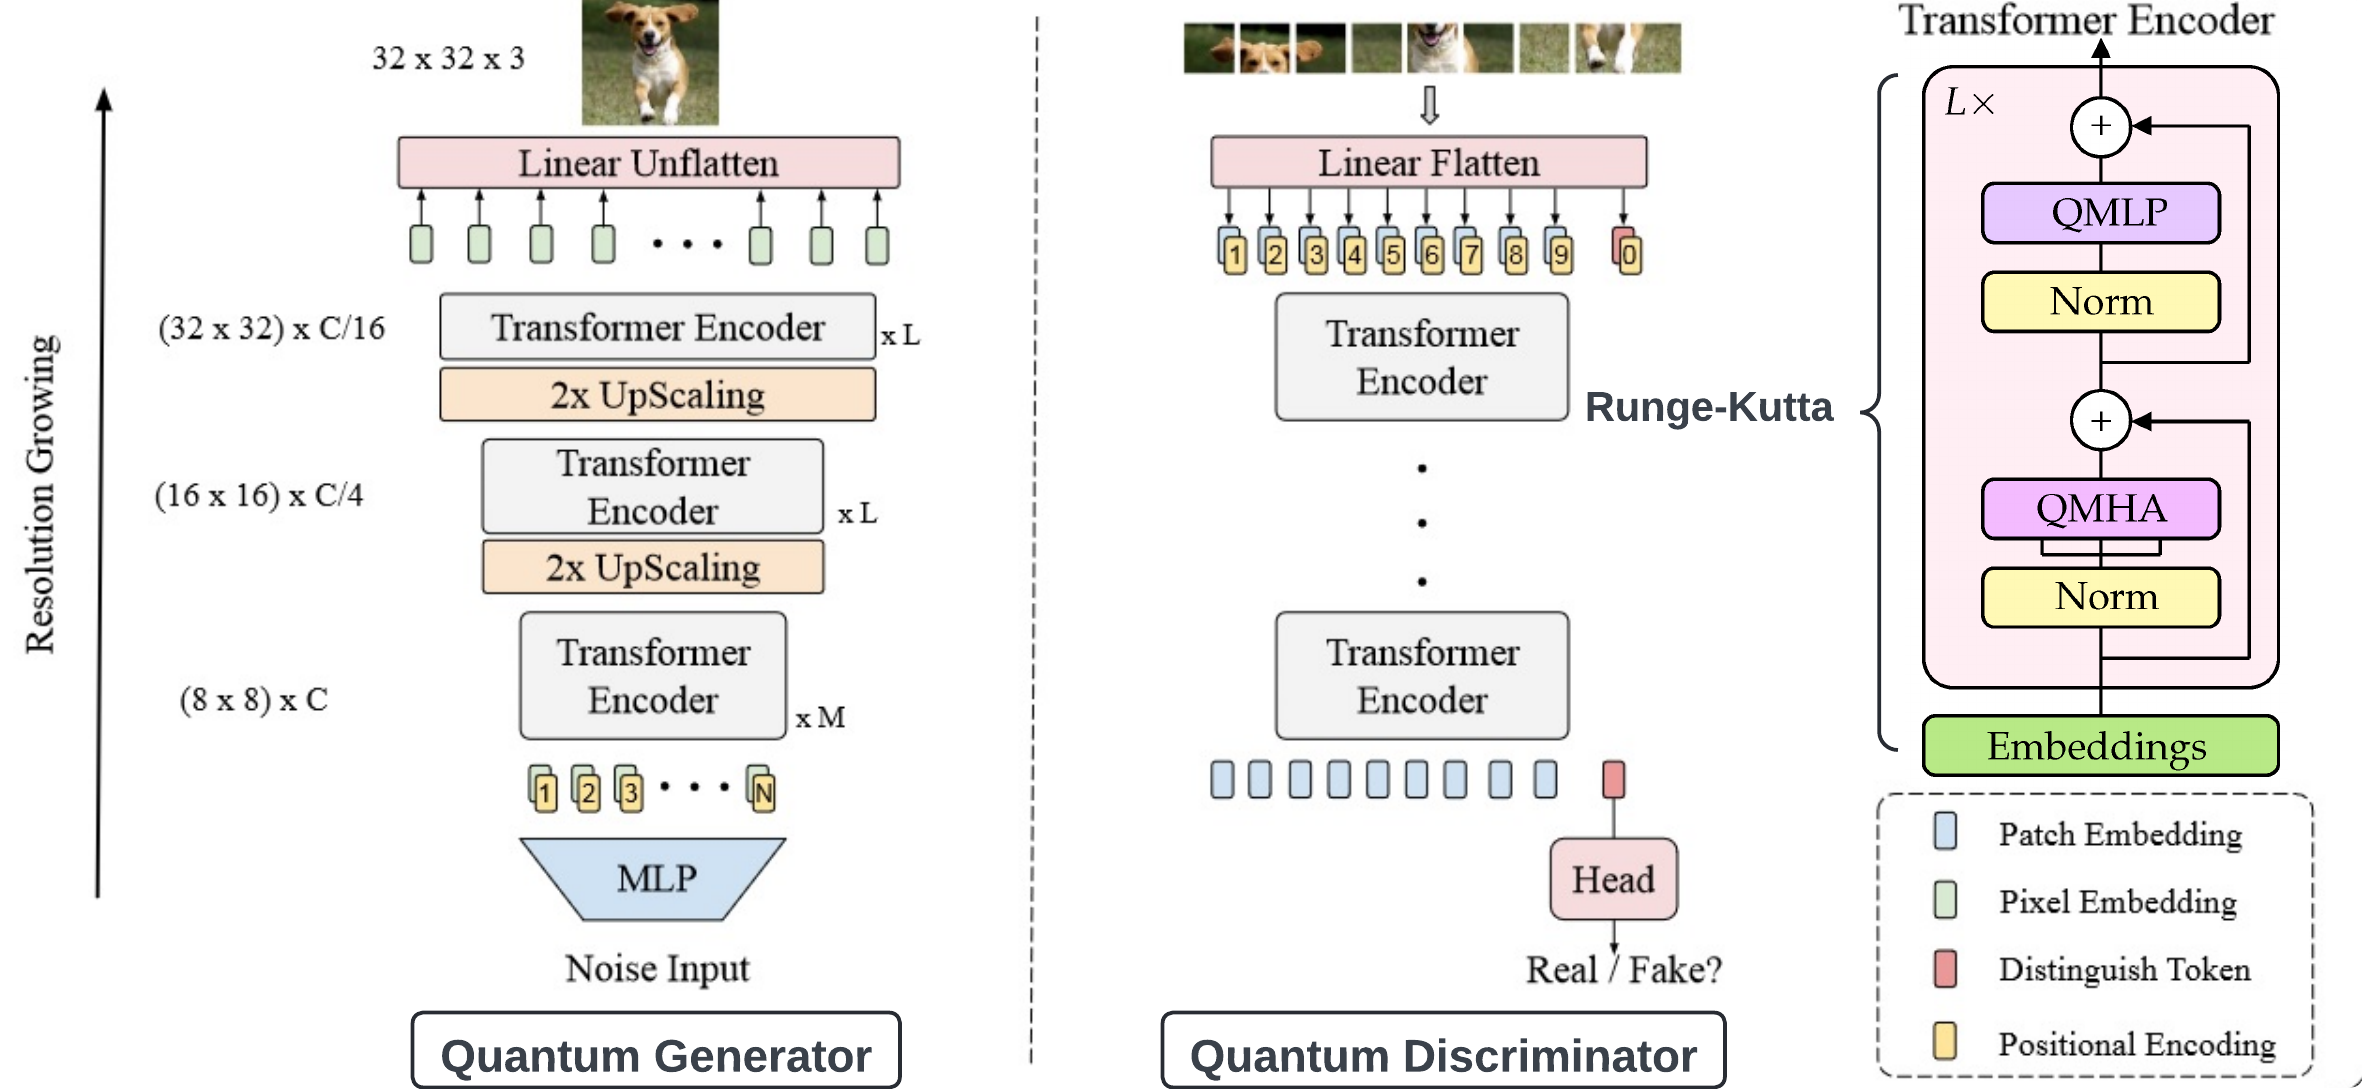
\includegraphics[scale=0.138]{./pics/Blank diagram - Page 1 (2).png}
      \caption[The QRKT-GAN Architecture]{The QRKT-GAN Architecture. Image inspired from~\cite{Comajoan_Cara_2024, jiang2021transgan}}
      \label{fig:p5}
    \end{figure}
  }
\end{frame}

\section{Results}

\begin{frame}{MNIST Classification}
  \visible<2->{
    \begin{figure}[th]
      \centering
      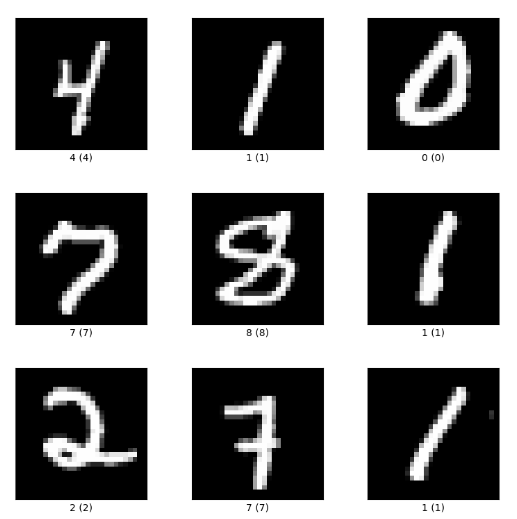
\includegraphics[scale=0.38]{./pics/mnist.png}
      \caption[Examples from MNIST]{Examples from MNIST\protect\footnotemark}
      \label{fig:p14}
    \end{figure}
  }
  \footnotetext{\url{https://www.tensorflow.org/datasets/catalog/mnist}}
\end{frame}

\begin{frame}
  \begin{figure}[th]
    \centering
    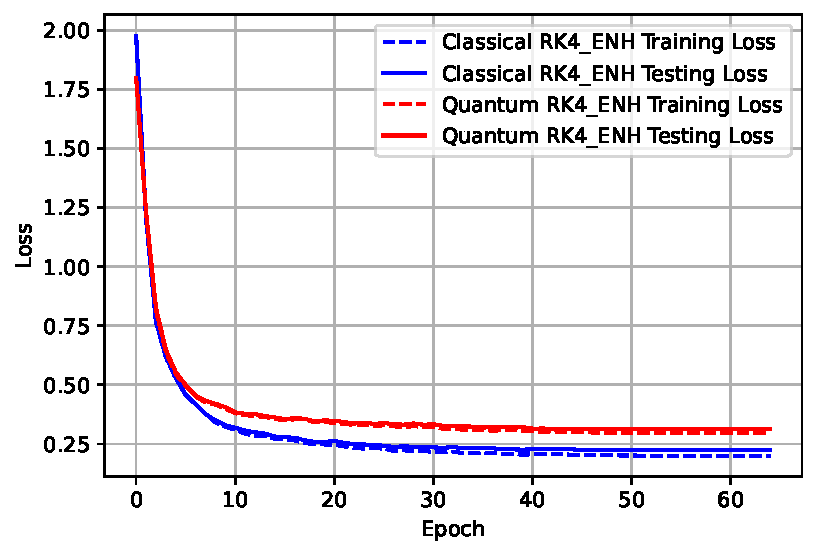
\includegraphics[scale=0.7]{./pics/new_pdf_graphs/hybrid/alternative_hybrid_transfomer_loss_mnist_rk4_enh.pdf}
    \caption[Cross-entropy loss evolution during learning]{Cross-entropy loss evolution during learning}
    \label{fig:p26}
  \end{figure}
\end{frame}

\begin{frame}
  \begin{figure}
    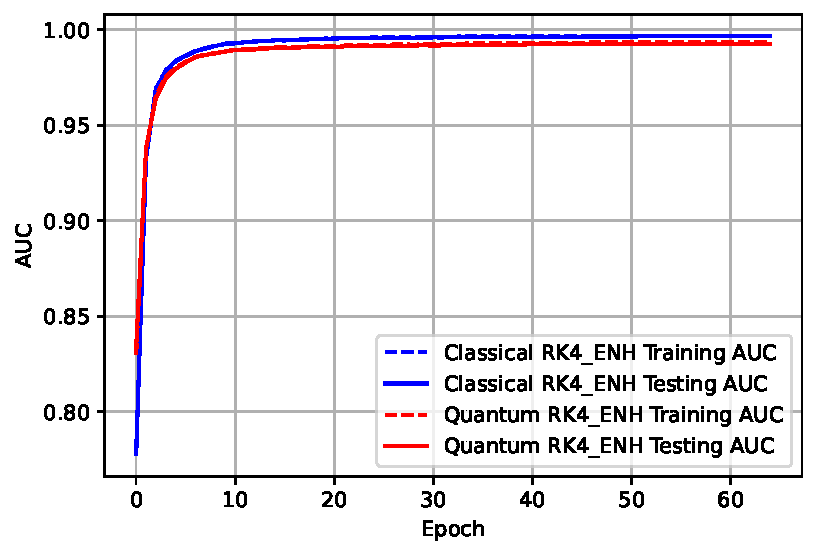
\includegraphics[scale=0.7]{./pics/new_pdf_graphs/hybrid/hybrid_auc_mnist_rk4.pdf}
    \caption[AUC score evolution during learning]{AUC score evolution during learning}
    \label{fig:p27}
  \end{figure}
\end{frame}

\begin{frame}
  \textbf{Configurations}:
  \bigskip
  \visible<2->{
    \begin{itemize}
      \item \textbf{Patch Size}: 14
      \item \textbf{Hidden Size}: 6
      \item \textbf{Classical and Quantum ODE-Transformer Blocks}: 3
      \item \textbf{Classical and Quantum Attention Heads}: 2
      \item \textbf{Hidden QMLP Size}: 3
    \end{itemize}
  }
  \visible<3->{
    \begin{table}[th]
      \small
      \linespread{1}
      \centering
      \resizebox{1.05\textwidth}{!}{ % Adjust the scaling factor as needed
        \begin{tabular}{|l|c|c|c|c|c|c|}
          \hline
          \textbf{ODE} & \textbf{Train Time (s)} & \textbf{Accuracy} & \textbf{F1 Score} & \textbf{Best AUC Epoch} & \textbf{\# Parameters} & \textbf{\# Qubits} \\
          \hline
          RK4\_ENH     & 1842.04                 & 95\%              & 95\%              & 54                      & 5971                   & -                  \\
          QRK4\_ENH    & 3539.44                 & 91\%              & 91\%              & 48                      & 3520                   & 357                \\
          \hline
        \end{tabular}
      }
      \caption{MNIST metrics for the quantum and classical configurations}
    \end{table}
  }
\end{frame}


\begin{frame}{CIFAR-10 Classification}
  \visible<2->{
    \begin{figure}[th]
      \centering
      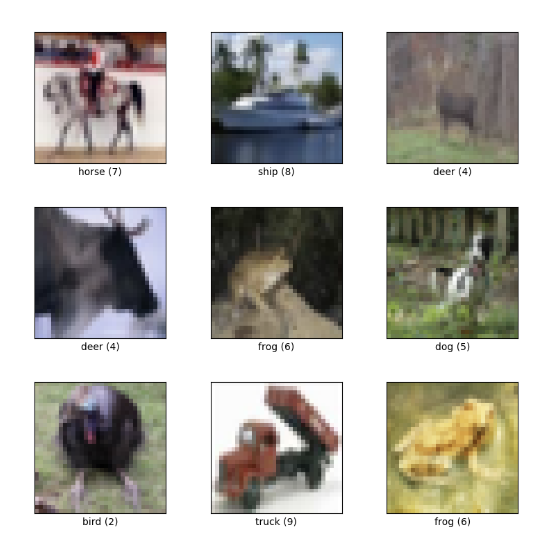
\includegraphics[scale=0.35]{./pics/cifar10.png}
      \caption[Examples from CIFAR-10]{Examples from CIFAR-10\protect\footnotemark}
      \label{fig:p28}
    \end{figure}
    \footnotetext{\url{https://www.tensorflow.org/datasets/catalog/cifar10}}
  }
\end{frame}

\begin{frame}
  \begin{figure}[th]
    \centering
    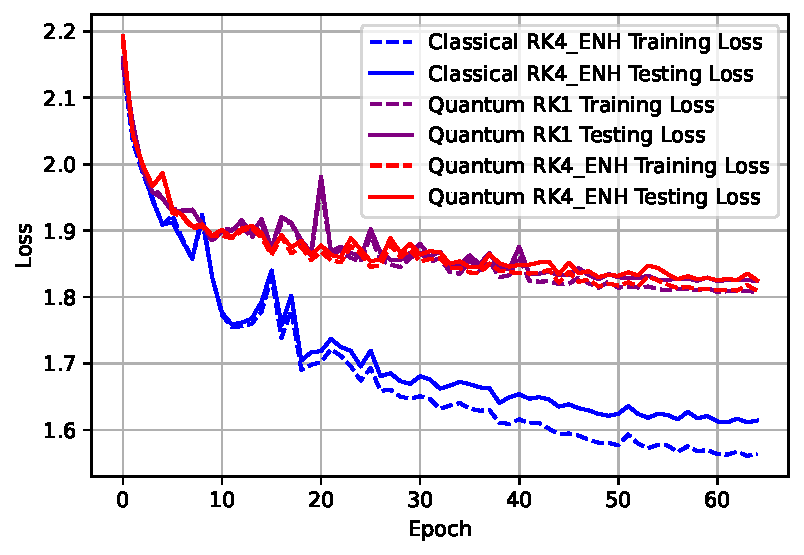
\includegraphics[scale=0.7]{./pics/new_pdf_graphs/hybrid/hybrid_transfomer_loss_cifar10_rk4_enh.pdf}
    \caption[Cross-entropy loss evolution during learning]{Cross-entropy loss evolution during learning}
    \label{fig:p26}
  \end{figure}
\end{frame}

\begin{frame}
  \begin{figure}
    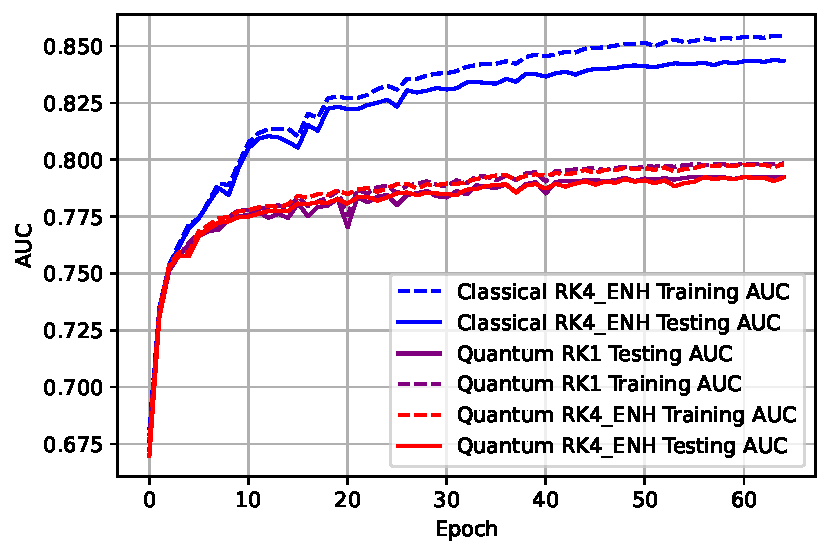
\includegraphics[scale=0.7]{./pics/new_pdf_graphs/hybrid/hybrid_auc_cifar10_.pdf}
    \caption[AUC score evolution during learning]{AUC score evolution during learning}
    \label{fig:p27}
  \end{figure}
\end{frame}

\begin{frame}
  \textbf{Configurations}:
  \bigskip
  \visible<2->{
    \begin{itemize}
      \item \textbf{Patch Size}: 16
      \item \textbf{Hidden Size}: 12
      \item \textbf{Classical and Quantum ODE-Transformer Blocks}: 1
      \item \textbf{Classical and Quantum Attention Heads}: 6
      \item \textbf{Hidden QMLP Size}: 6
    \end{itemize}
  }
  \visible<3->{
    \begin{table}[th]\small\linespread{1}
      \label{tab:hybrid_MNIST}
      \centering
      \resizebox{1.05\textwidth}{!}{\begin{tabular}{|l|c|c|c|c|c|c|}
          \hline
          \textbf{ODE} & \textbf{Train Time (s)} & \textbf{Accuracy} & \textbf{F1 Score} & \textbf{Best AUC Epoch} & \textbf{\# Parameters} & \textbf{\# Qubits} \\
          \hline
          RK4\_ENH     & 1685.04                 & 42\%              & 42\%              & 65                      & 33634                  & -                  \\
          QRK4\_ENH    & 16724.79                & 34\%              & 33\%              & 61                      & 20590                  & 390                \\
          QRK1         & 10909.40                & 33\%              & 33\%              & 56                      & 20590                  & 336                \\
          \hline
        \end{tabular}
      }
      \caption{CIFAR-10 metrics for the quantum and classical configurations}
    \end{table}
  }
\end{frame}

\begin{frame}{IMDb Classification}
  \visible<2->{
    \begin{table}[h!]
      \centering
      \resizebox{1\textwidth}{!}{\begin{tabular}{|c|p{12cm}|}
          \hline
          \textbf{Label} & \textbf{Text}                                                                                                                                                                                                                                                                                                                                                                                          \\
          \hline
          0 (neg)        & "I have been known to fall asleep during films, but this is usually due to a combination of things including, really tired, being warm and comfortable on the settee and having just eaten a lot. However on this occasion I fell asleep because the film was rubbish [...]"                                                                                                                           \\
          \hline
          1 (pos)        & "This is a film which should be seen by anybody interested in, effected by, or suffering from an eating disorder. It is an amazingly accurate and sensitive portrayal of bulimia in a teenage girl, its causes and its symptoms. The girl is played by one of the most brilliant young actresses working in cinema today, Alison Lohman, who was later so spectacular in 'Where the Truth Lies' [...]" \\
          \hline
        \end{tabular}
      }
      \caption{Movie Reviews\protect\footnotemark}
      \label{table:negative_reviews}
    \end{table}\footnotetext{https://www.tensorflow.org/datasets/catalog/imdb\_reviews}

  }
\end{frame}

\begin{frame}
  \begin{figure}[th]
    \centering
    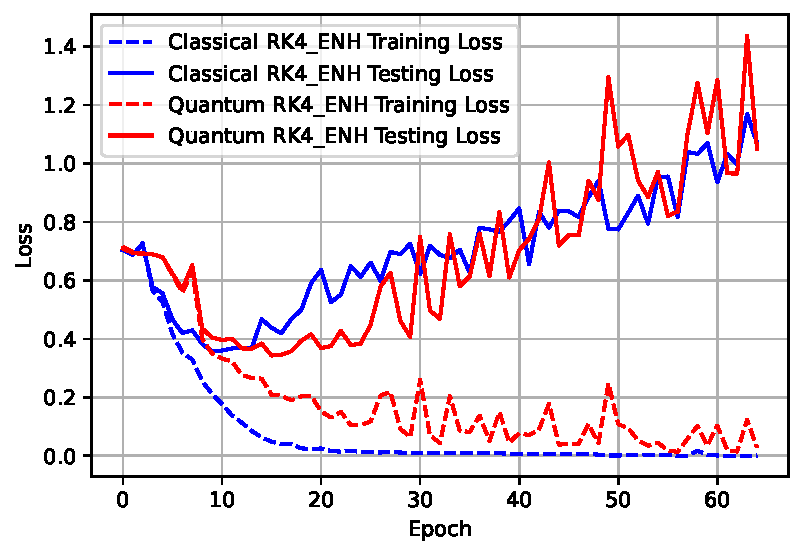
\includegraphics[scale=0.7]{./pics/new_pdf_graphs/hybrid/hybrid_transfomer_loss_imdb_rk4_enh.pdf}
    \caption[Cross-entropy loss evolution during learning]{Cross-entropy loss evolution during learning}
    \label{fig:p26}
  \end{figure}
\end{frame}

\begin{frame}
  \begin{figure}
    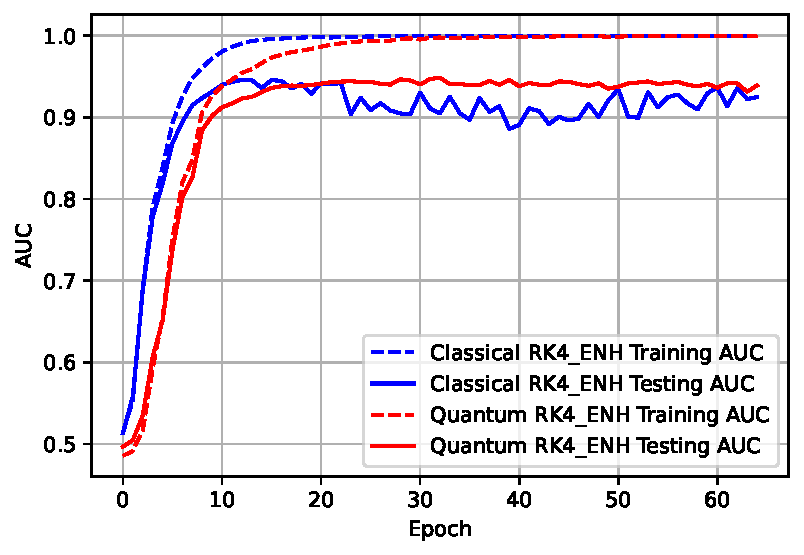
\includegraphics[scale=0.7]{./pics/new_pdf_graphs/hybrid/hybrid_auc_imdb_.pdf}
    \caption[AUC score evolution during learning]{AUC score evolution during learning}
    \label{fig:p27}
  \end{figure}
\end{frame}

\begin{frame}
  \textbf{Configurations}:
  \bigskip
  \visible<2->{
    \begin{itemize}
      \item \textbf{Max sequence length}: 512
      \item \textbf{Classical / Quantum Hidden Size}: 12 / 6
      \item \textbf{Classical / Quantum ODE-Transformer Blocks}: 1 / 1
      \item \textbf{Classical / Quantum Attention Heads}: 6 / 2
      \item \textbf{Classical / Quantum Hidden MLP Size}: 6 / 3
    \end{itemize}
  }
  \visible<3->{
    \begin{table}[th]\small\linespread{1}
      \label{tab:classical_CIFAR_1}
      \centering
      \resizebox{1.05\textwidth}{!}{\begin{tabular}{|l|c|c|c|c|c|c|}
          \hline
          \textbf{ODE} & \textbf{Train Time (s)} & \textbf{Accuracy} & \textbf{F1 Score} & \textbf{Best AUC Epoch} & \textbf{\# Parameters} & \textbf{\# Qubits} \\
          \hline
          RK4\_ENH     & 3328.61                 & 85\%              & 85\%              & 13                      & 499316                 & -                  \\
          QRK4\_ENH    & 9033.13                 & \textbf{85}\%     & \textbf{85}\%     & 33                      & \textbf{243896}        & 141                \\
          \hline
        \end{tabular}
      }
      \caption{IMDb metrics for the classical and quantum configurations}
    \end{table}
  }
\end{frame}

\begin{frame}{Synthetic Data Generation}
  \visible<2->{
    \begin{table}[h!]
      \centering
      \resizebox{0.7\textwidth}{!}{\begin{tabular}{|c|c|c|}
          \hline
          \textbf{Metric}                  & \textbf{QRKT-GAN} & \textbf{TransGAN} \\
          \hline
          Inception Score (IS)             & 74.89             & 52.31             \\
          \hline
          Fréchet Inception Distance (FID) & 66.78             & 46.97             \\
          \hline
        \end{tabular}
      }
      \caption{Performance Metrics for TransGAN and QRKT-GAN on CIFAR-10}
      \label{table:performance_metrics}
    \end{table}
  }
  \visible<3->{
    \begin{figure}[th]
      \centering
      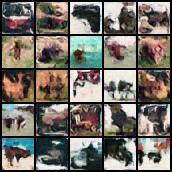
\includegraphics[scale=0.6]{./pics/generated_img_39_1600.jpg}
      \caption[Generated Images using QRKT-GAN]{Generated Images using QRKT-GAN}
      \label{fig:p41}
    \end{figure}
  }
\end{frame}

\begin{frame}
  Technologies used for QRKT-GAN:
  \smallskip
  \smallskip
  \visible<2->{
    \begin{itemize}
      \item JAX~\cite{bradbury2018jax} and Flax~\cite{heek2020flax}
      \item Tensorflow Quantum~\cite{broughton2020tensorflow}
      \item Qiskit~\cite{cross2018ibm}
      \item Pytorch~\cite{imambi2021pytorch}
      \item Tensor Circuit~\cite{Zhang_2023}
    \end{itemize}
  }
\end{frame}

\section{Conclusion}
\begin{frame}{Conclusion}
  Keywords:
  \visible<2->{
    \begin{itemize}
      \item Deep Learning
      \item Transformers
      \item GANs
      \item Runge-Kutta
      \item Quantum
      \item \alert{Optimization}
    \end{itemize}
  }
  \smallskip
  \smallskip
  \centering
  \Huge
  \visible<3->{$| \text{Thank you!} \rangle$}
\end{frame}

\section{References}
\begin{frame}[allowframebreaks]{References}
  \bibliographystyle{unsrt}
  \bibliography{bibliography}
\end{frame}

\end{document}
